% vim:encoding=utf8 ft=tex sts=2 sw=2 et:

\documentclass{classrep}
\usepackage[utf8]{inputenc}
\usepackage{color}
\usepackage{graphicx}
\usepackage{float}

\studycycle{Informatyka, studia dzienne, mgr II st.}
\coursesemester{II}

\coursename{Rozpoznawanie obrazów}
\courseyear{2017/2018}

\courseteacher{dr inż. Bartłomiej Stasiak}
\coursegroup{wtorek, 12:00}

\author{
  \studentinfo{Hubert Marcinkowski}{214942} \and
  \studentinfo{Artur Wróblewski}{214985}
}

\title{Zadanie 2}

\begin{document}
\maketitle

\section{Wyniki}

Zgodnie z zaleceniami prowadzącego wprowadziliśmy normalizację obrazów wejściowych. Niestety wpłynęła ona negatywnie na otrzymane średnie wyników.

\begin{table}[h!]
  \centering
  \caption{Macierz pomyłek k-NN dla bazy znormalizowanych tekstur dla cech w dziedzinie czasu oraz częstotliwości oraz $k=11$. Średnia równa $76.50\%$}
  \label{tab:tab1}
  \begin{tabular}{|c|c|c|c|c|c|}
    \hline
	. & 0 & 1 & 2 & 3 & recall \\
    \hline
	0 & 152513 & 2139 & 7487 & 22147 & 82.75\\
    \hline
	1 & 161 & 177783 & 25865 & 767 & 86.90\\
	\hline
	2 & 9640 & 51712 & 133628 & 67 & 68.51\\
	\hline
	3 & 13625 & 5089 & 64373 & 137436 & 67.86\\   
    \hline
  \end{tabular}
\end{table}

\begin{table}[h!]
  \centering
  \caption{Macierz pomyłek k-NN dla bazy nieznormalizowanych tekstur dla cech w dziedzinie czasu oraz częstotliwości oraz $k=11$. Średnia równa $79.23\%$}
  \label{tab:tab1}
  \begin{tabular}{|c|c|c|c|c|c|}
    \hline
	. & 0 & 1 & 2 & 3 & recall \\
    \hline
	0 & 160791 & 920 & 13424 & 9151 & 87.25\\
    \hline
	1 & 168 & 175602 & 27804 & 1002 & 85.83\\
	\hline
	2 & 3977 & 22444 & 1667241 & 1385 & 85.74\\
	\hline
	3 & 32927 & 3958 & 47932 & 117706 & 58.11\\   
    \hline
  \end{tabular}
\end{table}

\begin{figure}[h!]
	\centering
  	
\includegraphics[width=\linewidth]{1.png}
	\caption{Wyniki klasyfikacji dla pierwszej tekstury. Od lewej: z normalizacją obrazów, bez normalizacji, etykiety docelowe.}
	\label{fig:widma}
\end{figure}

\begin{figure}[h!]
	\centering
  	
\includegraphics[width=\linewidth]{2.png}
	\caption{Wyniki klasyfikacji dla drugiej tekstury. Od lewej: z normalizacją obrazów, bez normalizacji, etykiety docelowe.}
	\label{fig:widma}
\end{figure}

\begin{figure}[h!]
	\centering
  	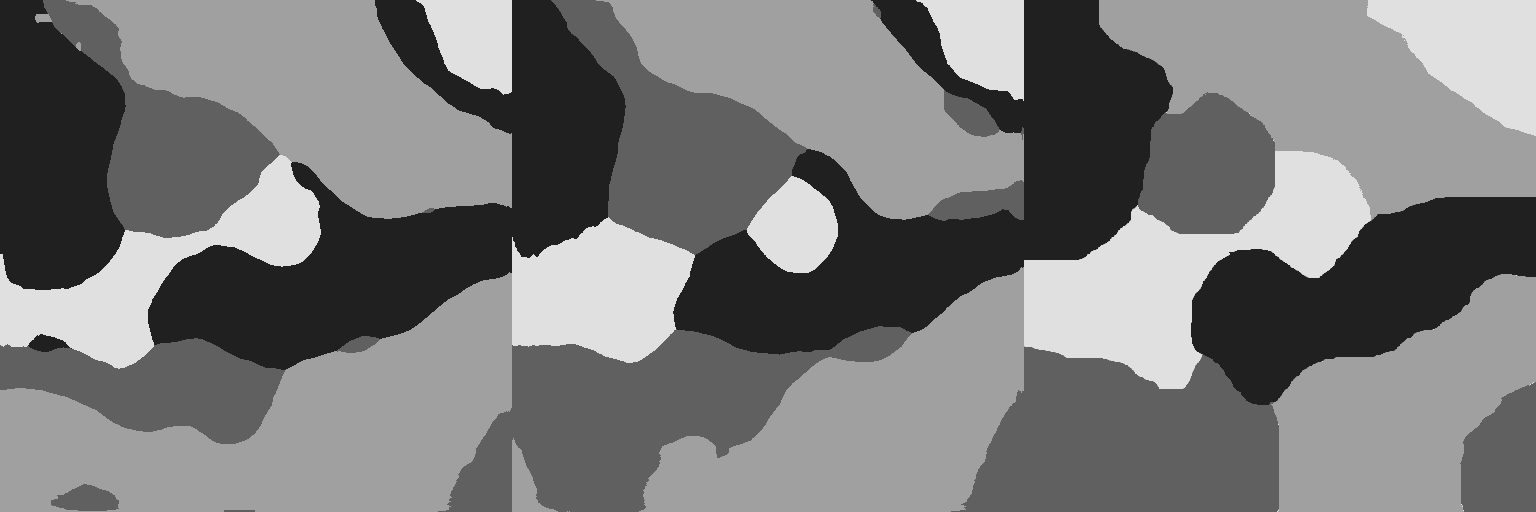
\includegraphics[width=\linewidth]{3.png}
	\caption{Wyniki klasyfikacji dla trzeciej tekstury. Od lewej: z normalizacją obrazów, bez normalizacji, etykiety docelowe.}
	\label{fig:widma}
\end{figure}

\end{document}
